\subsection{User Interfaces}
DREAM contains two main interfaces: mobile application and webapp interface.
In both interfaces, all three actors can perform the same operations.
However, it should be noted that certain features are more comfortable to use only from a certain interface.
The following mockups will give a more detailed description in terms of interfaces.

\begin{figure}[H]
  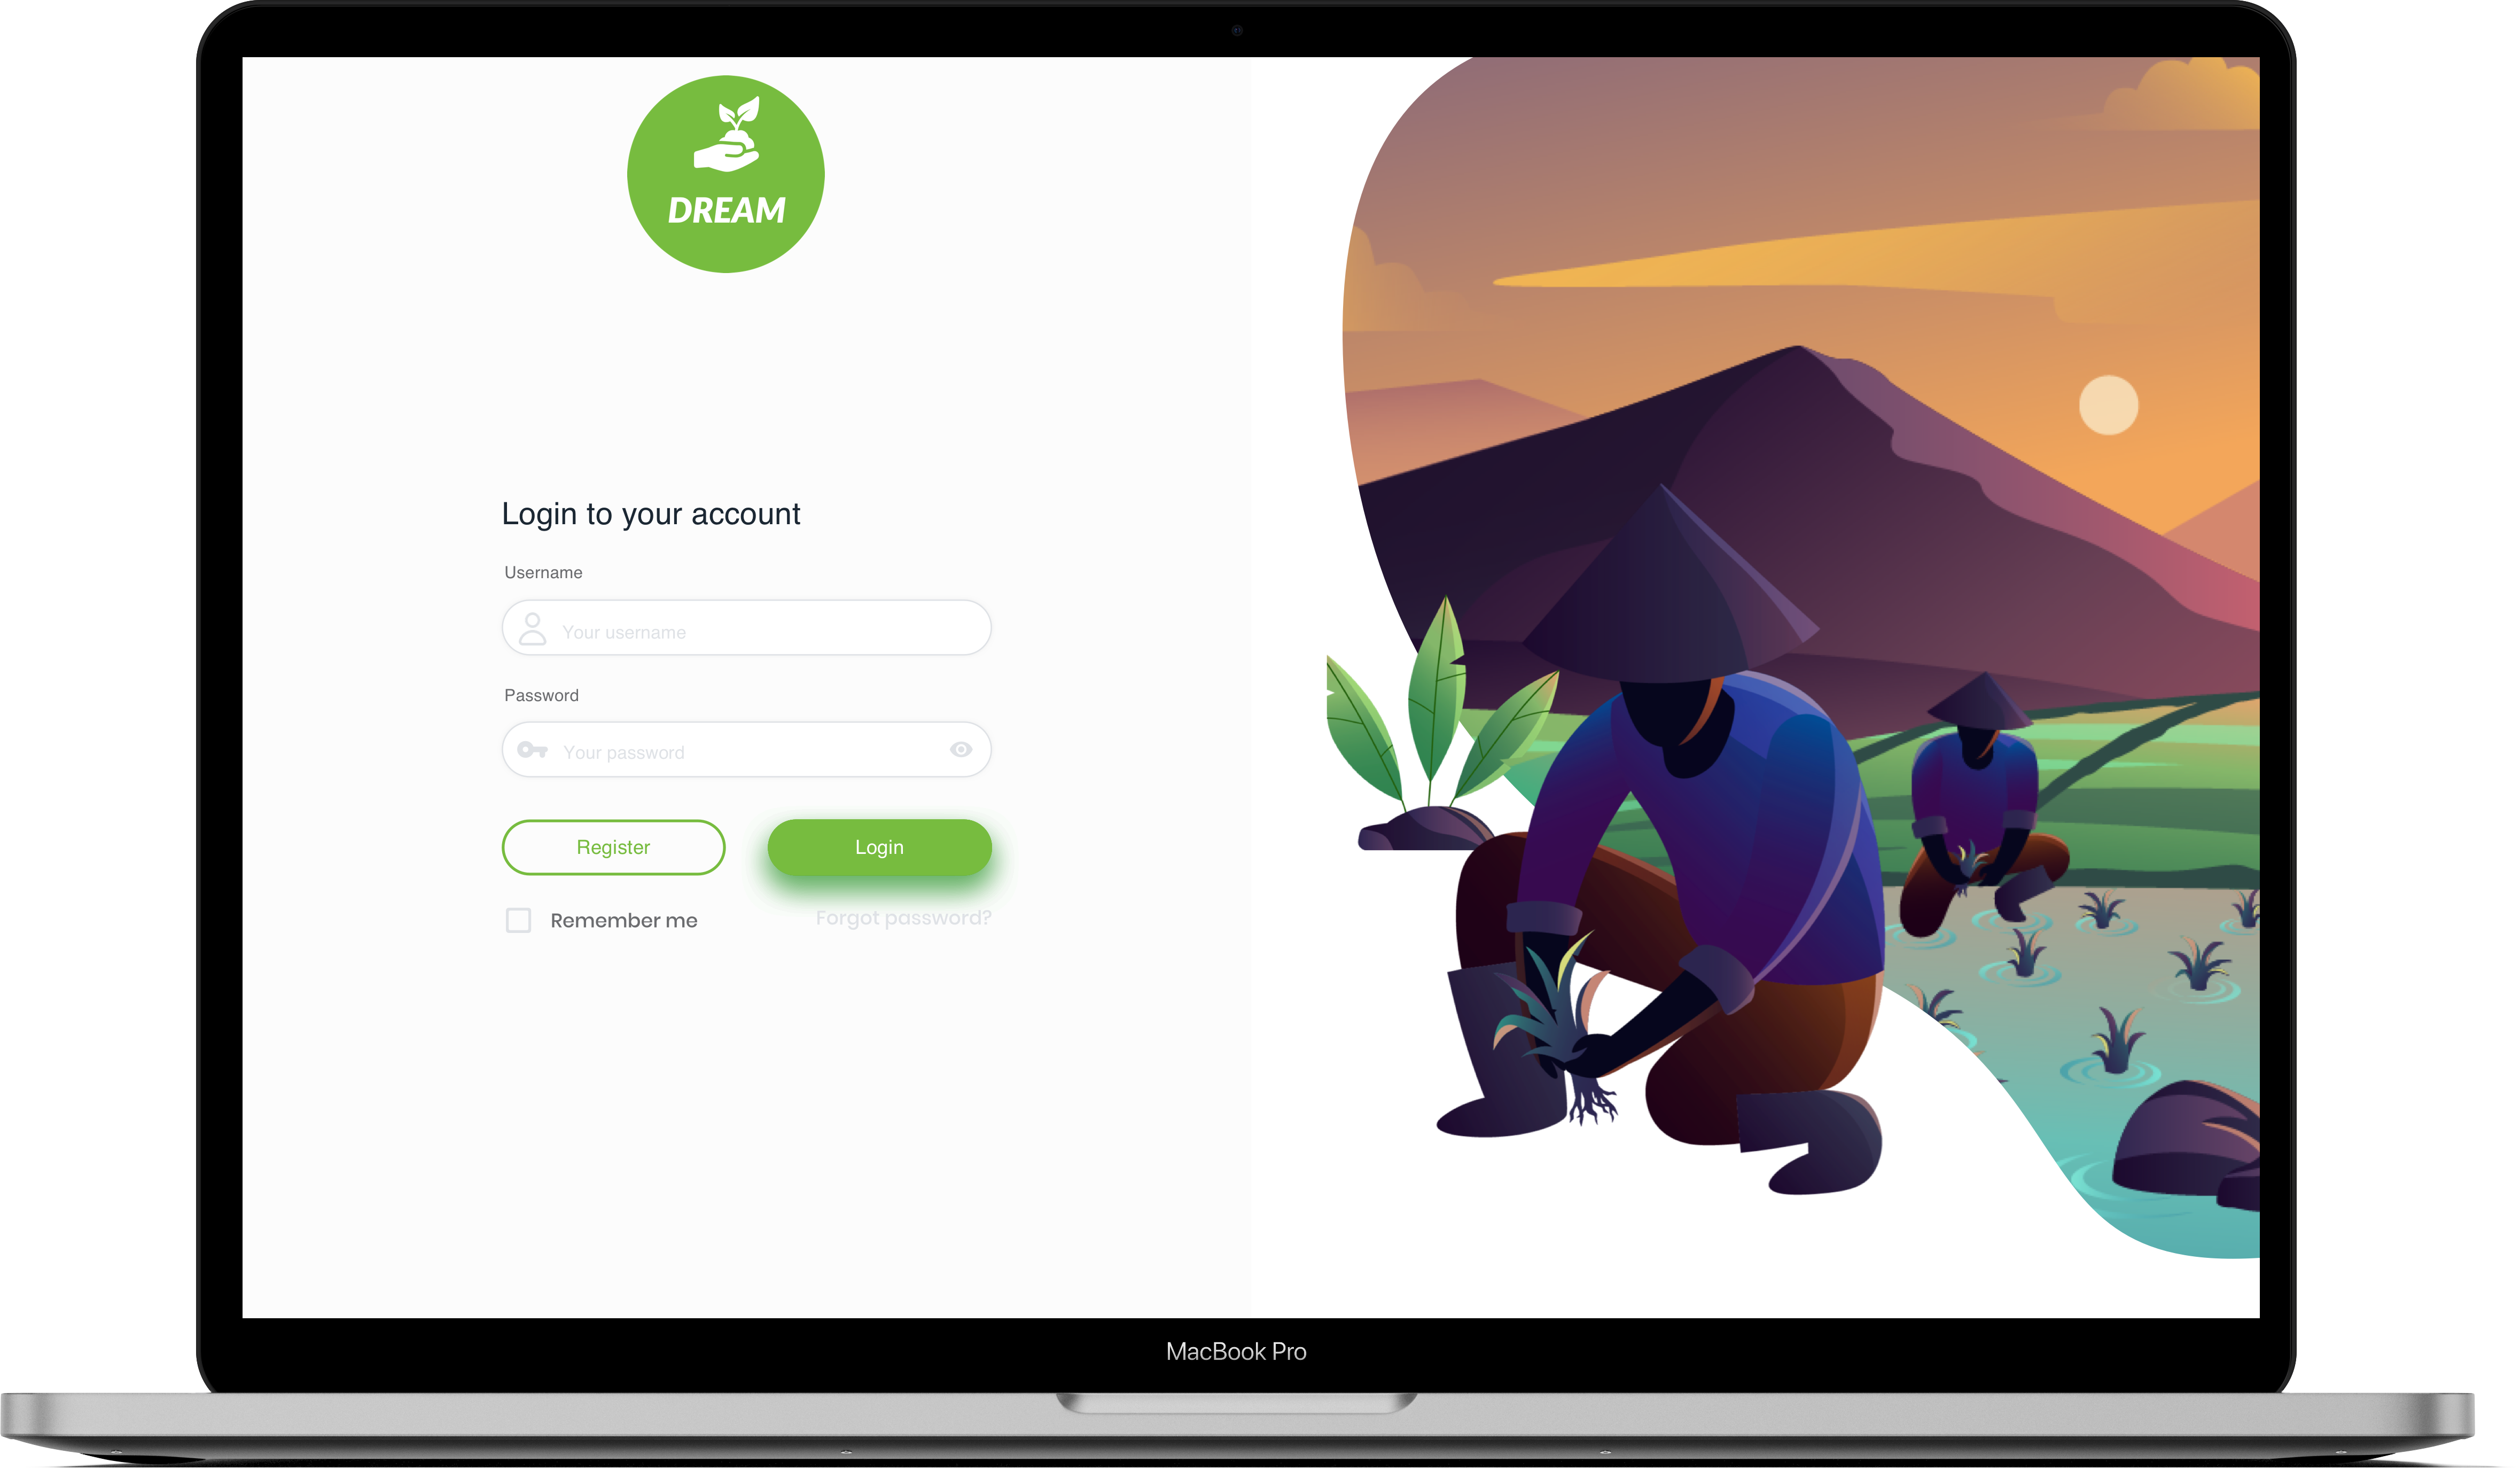
\includegraphics[width=140mm,scale=0.9]{./Images//Mocks/WebApp/Login.png}
  \caption{Login}
\end{figure}

\begin{itemize}
    \item \textbf{Website Login}\\ 
    \textcolor{red}{The three actors of DREAM can access to the application through this login page. If they do not yet have an account, they can simply access the registration page via an appropriate button}
\end{itemize}


\begin{figure}[H]
  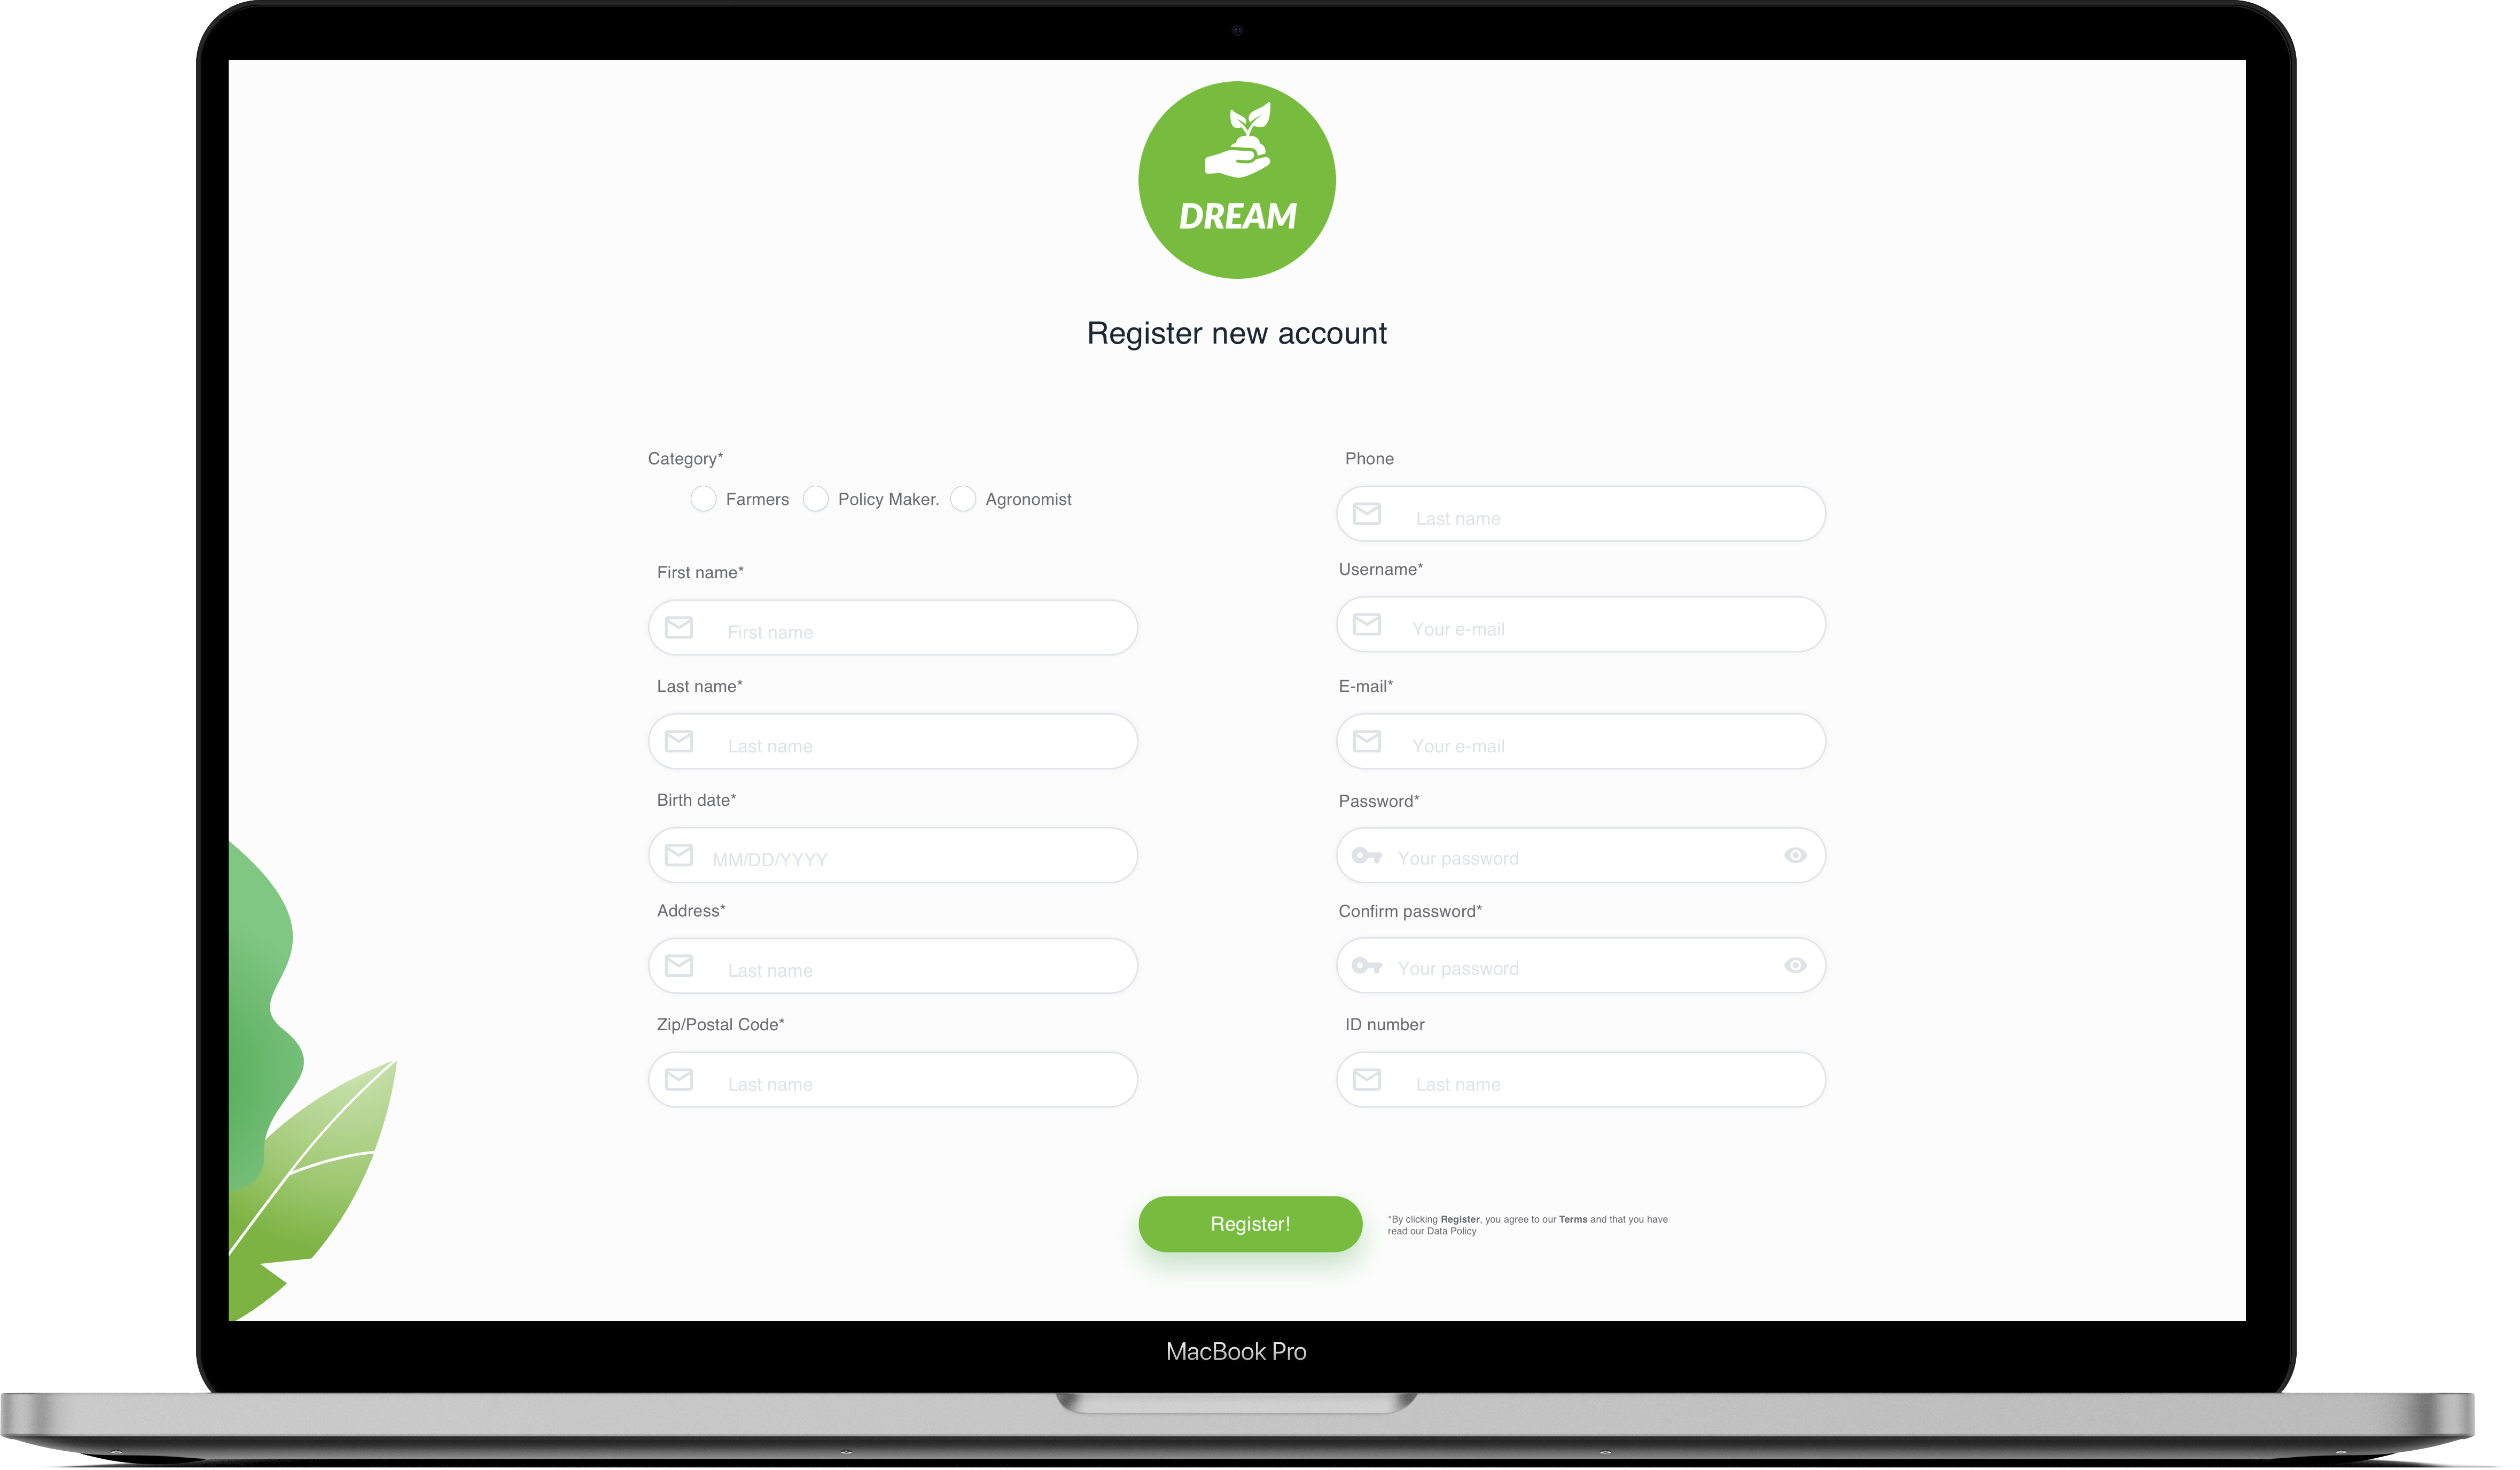
\includegraphics[width=140mm,scale=0.9]{./Images//Mocks/WebApp/Registration.png}
  \caption{Registration}
\end{figure}

\begin{itemize}
    \item \textbf{Website Registration}\\ 
    \textcolor{red}{The three actors can register to DREAM through this registration page, where there are some required fields, and registration is completed by accepting term and conditions}
\end{itemize}


\begin{figure}[H]
  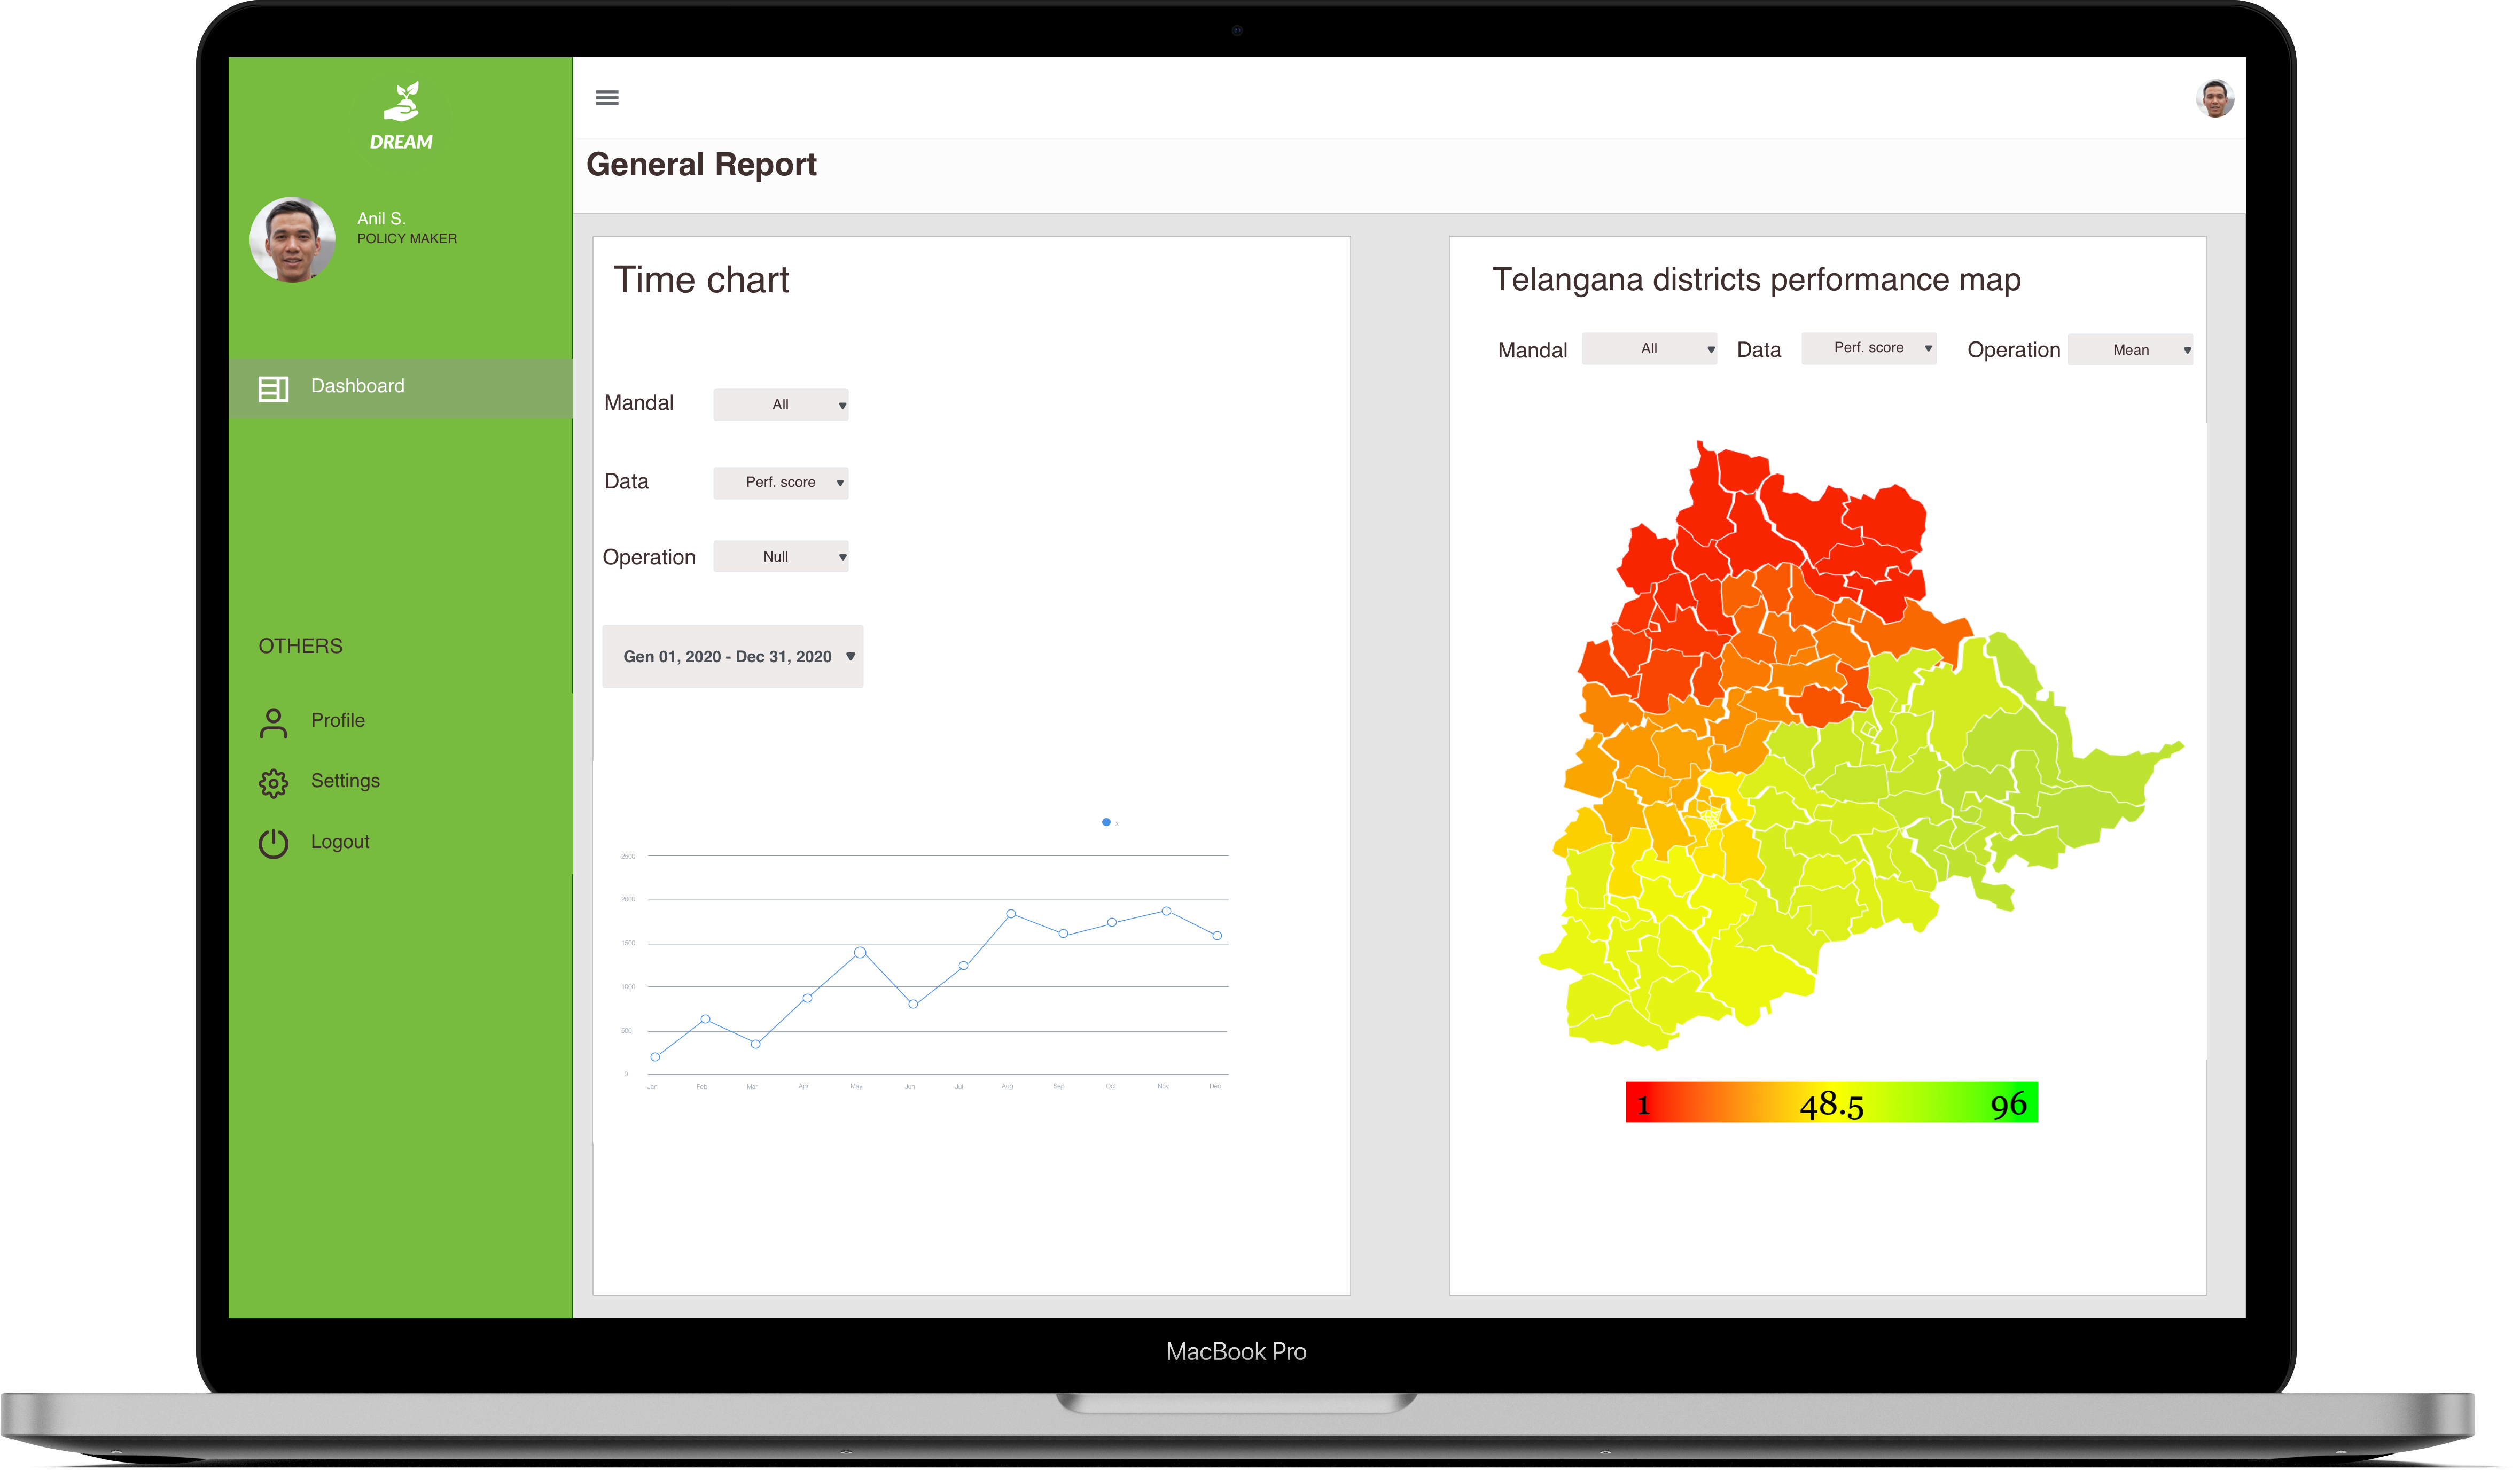
\includegraphics[width=140mm,scale=0.9]{./Images//Mocks/WebApp/PolicyMaker.png}
  \caption{PolicyMaker Homepage}
\end{figure}

\begin{itemize}
    \item \textbf{PolicyMaker Homepage}\\ 
    \textcolor{red}{This is PolicyMaker homepage (in \textit{Figure 3.3} called "Dashboard") where the he/she can generate a time chart according to some inputs, and can also visualize Telangana's farmers performance map using some filters as shown in the Figure 3.3}
\end{itemize}


\begin{figure}[H]
  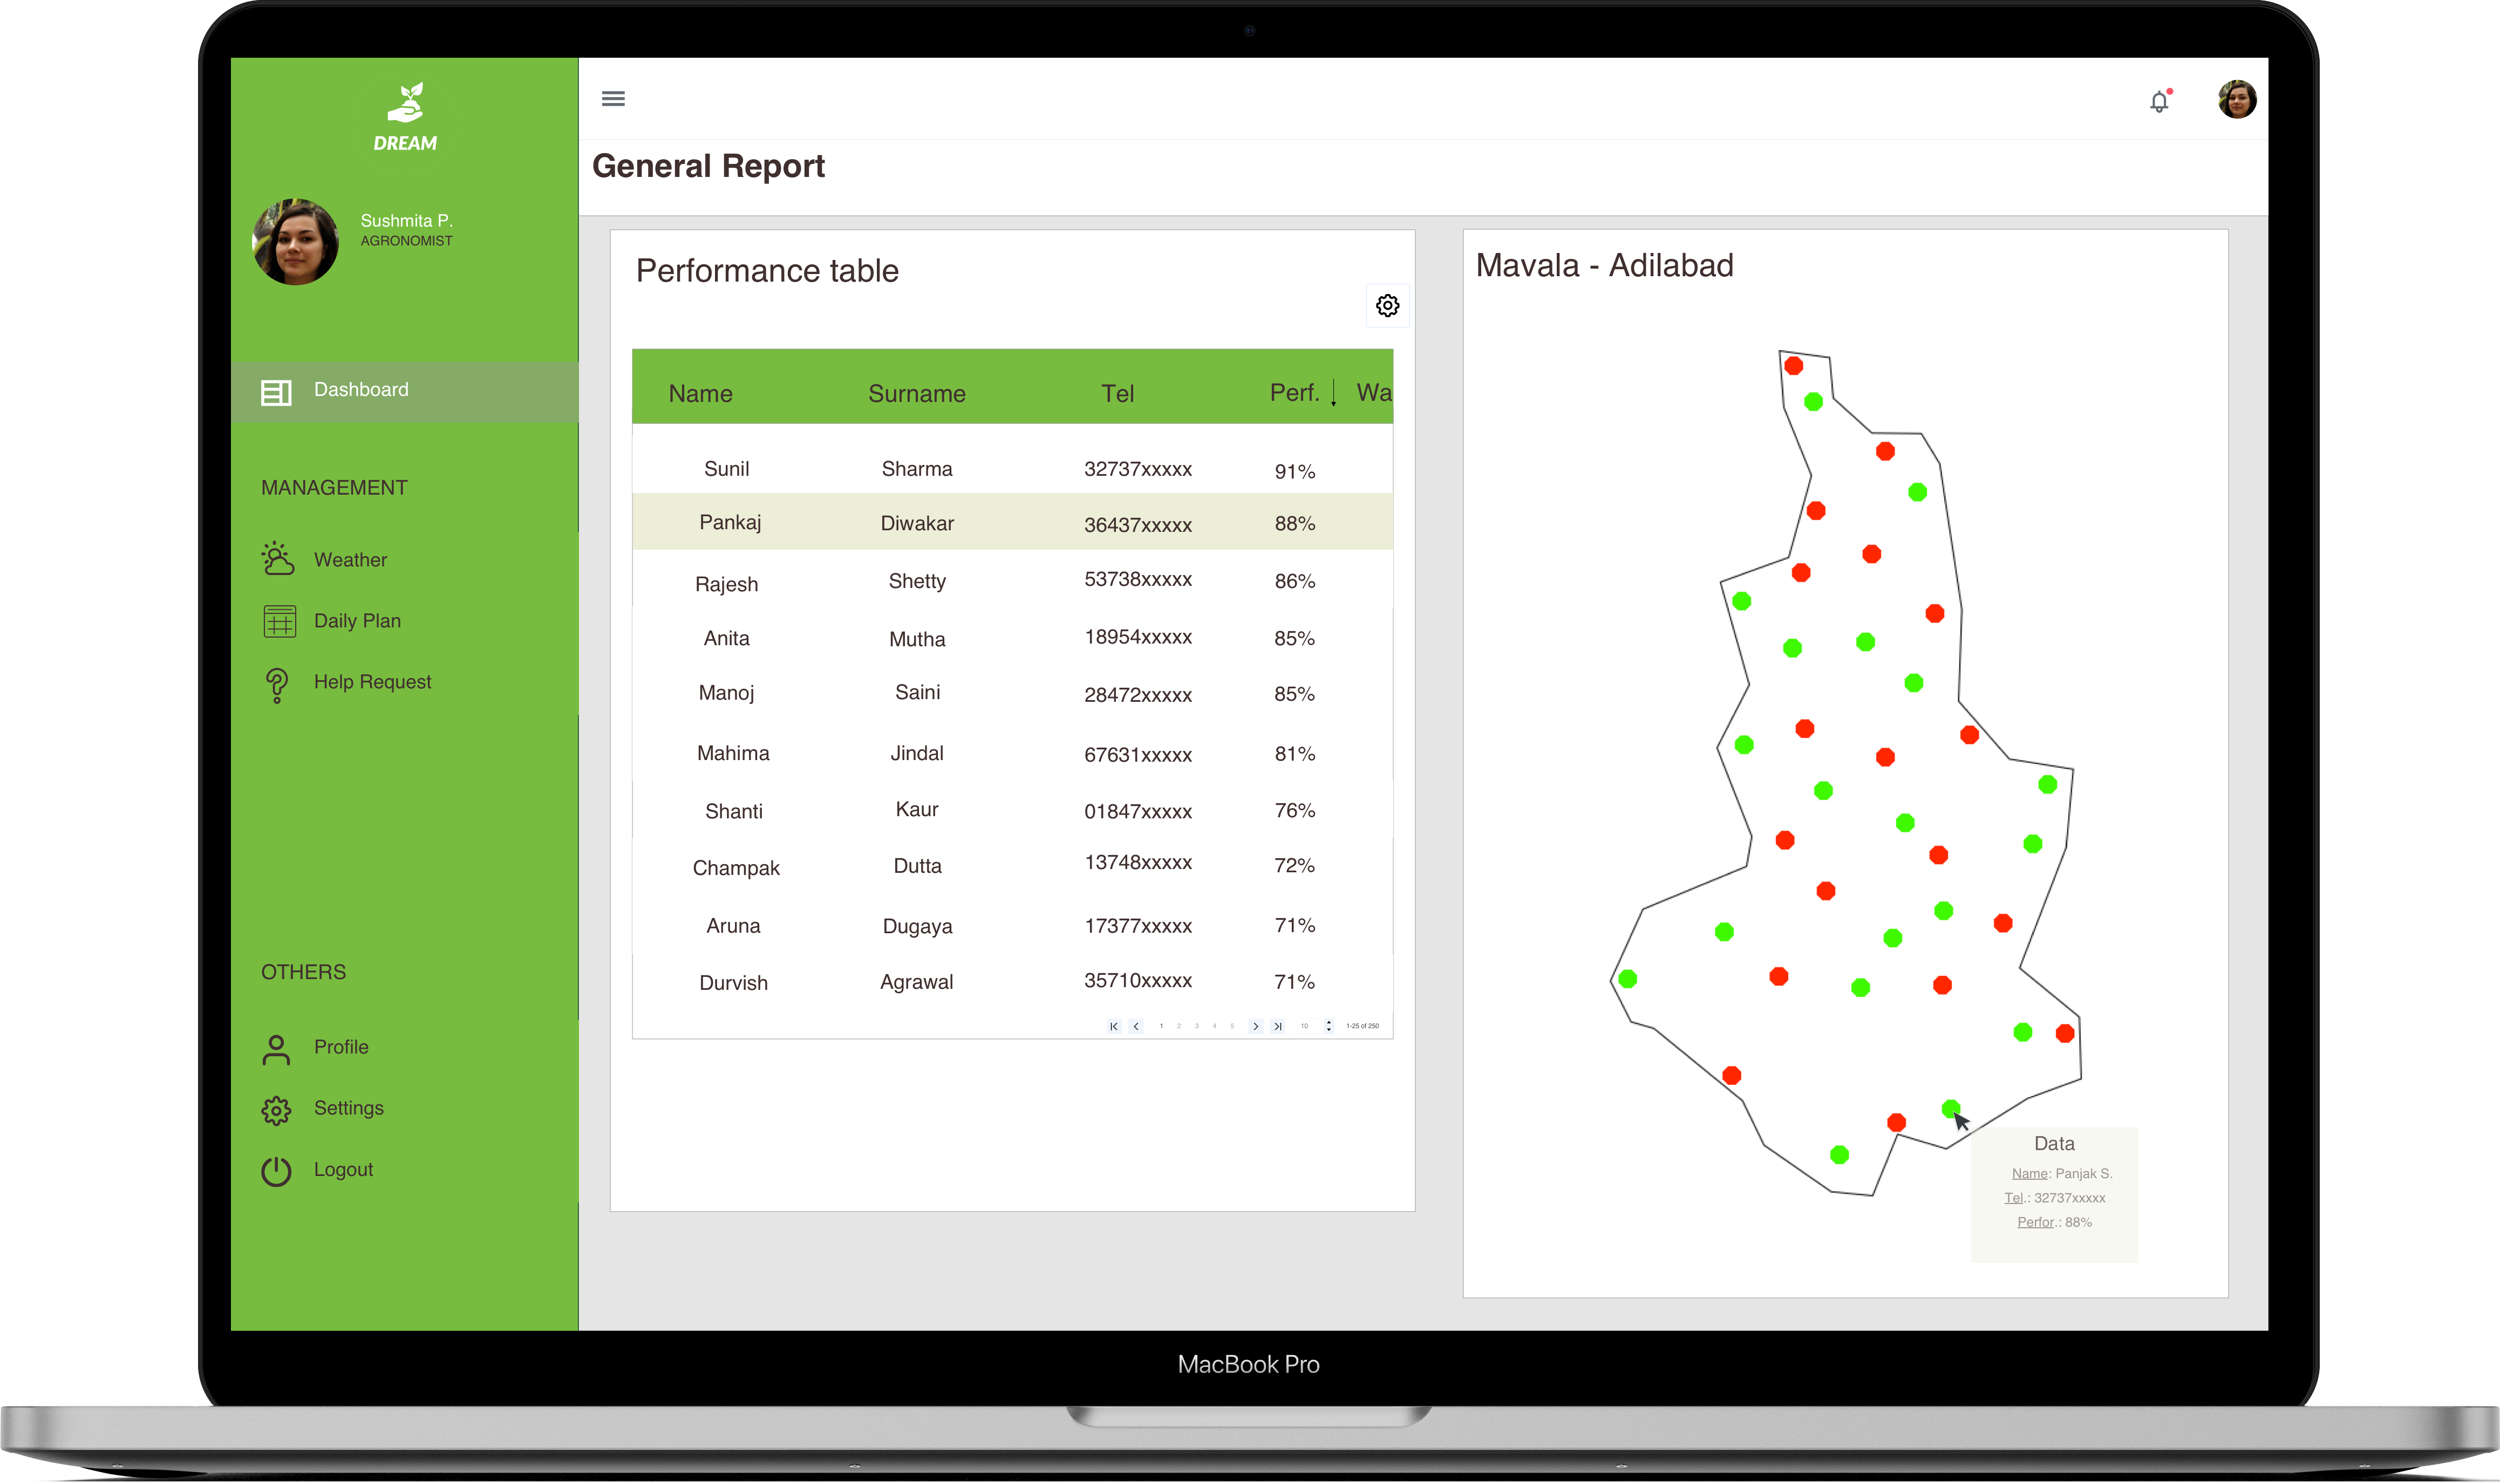
\includegraphics[width=140mm,scale=0.9]{./Images//Mocks/WebApp/Agronomist_Home.png}
  \caption{Agronomist Homepage}
\end{figure}

\begin{itemize}
    \item \textbf{Agronomist Homepage}\\ 
    \textcolor{red}{This is Agronomist homepage (in \textit{Figure 3.4} called "Dashboard") where he/she can view his/her mandal's farmer performance on a map, and the performance table, that resume, in ascending order (by performance), info's about farmers.}
\end{itemize}


\begin{figure}[H]
  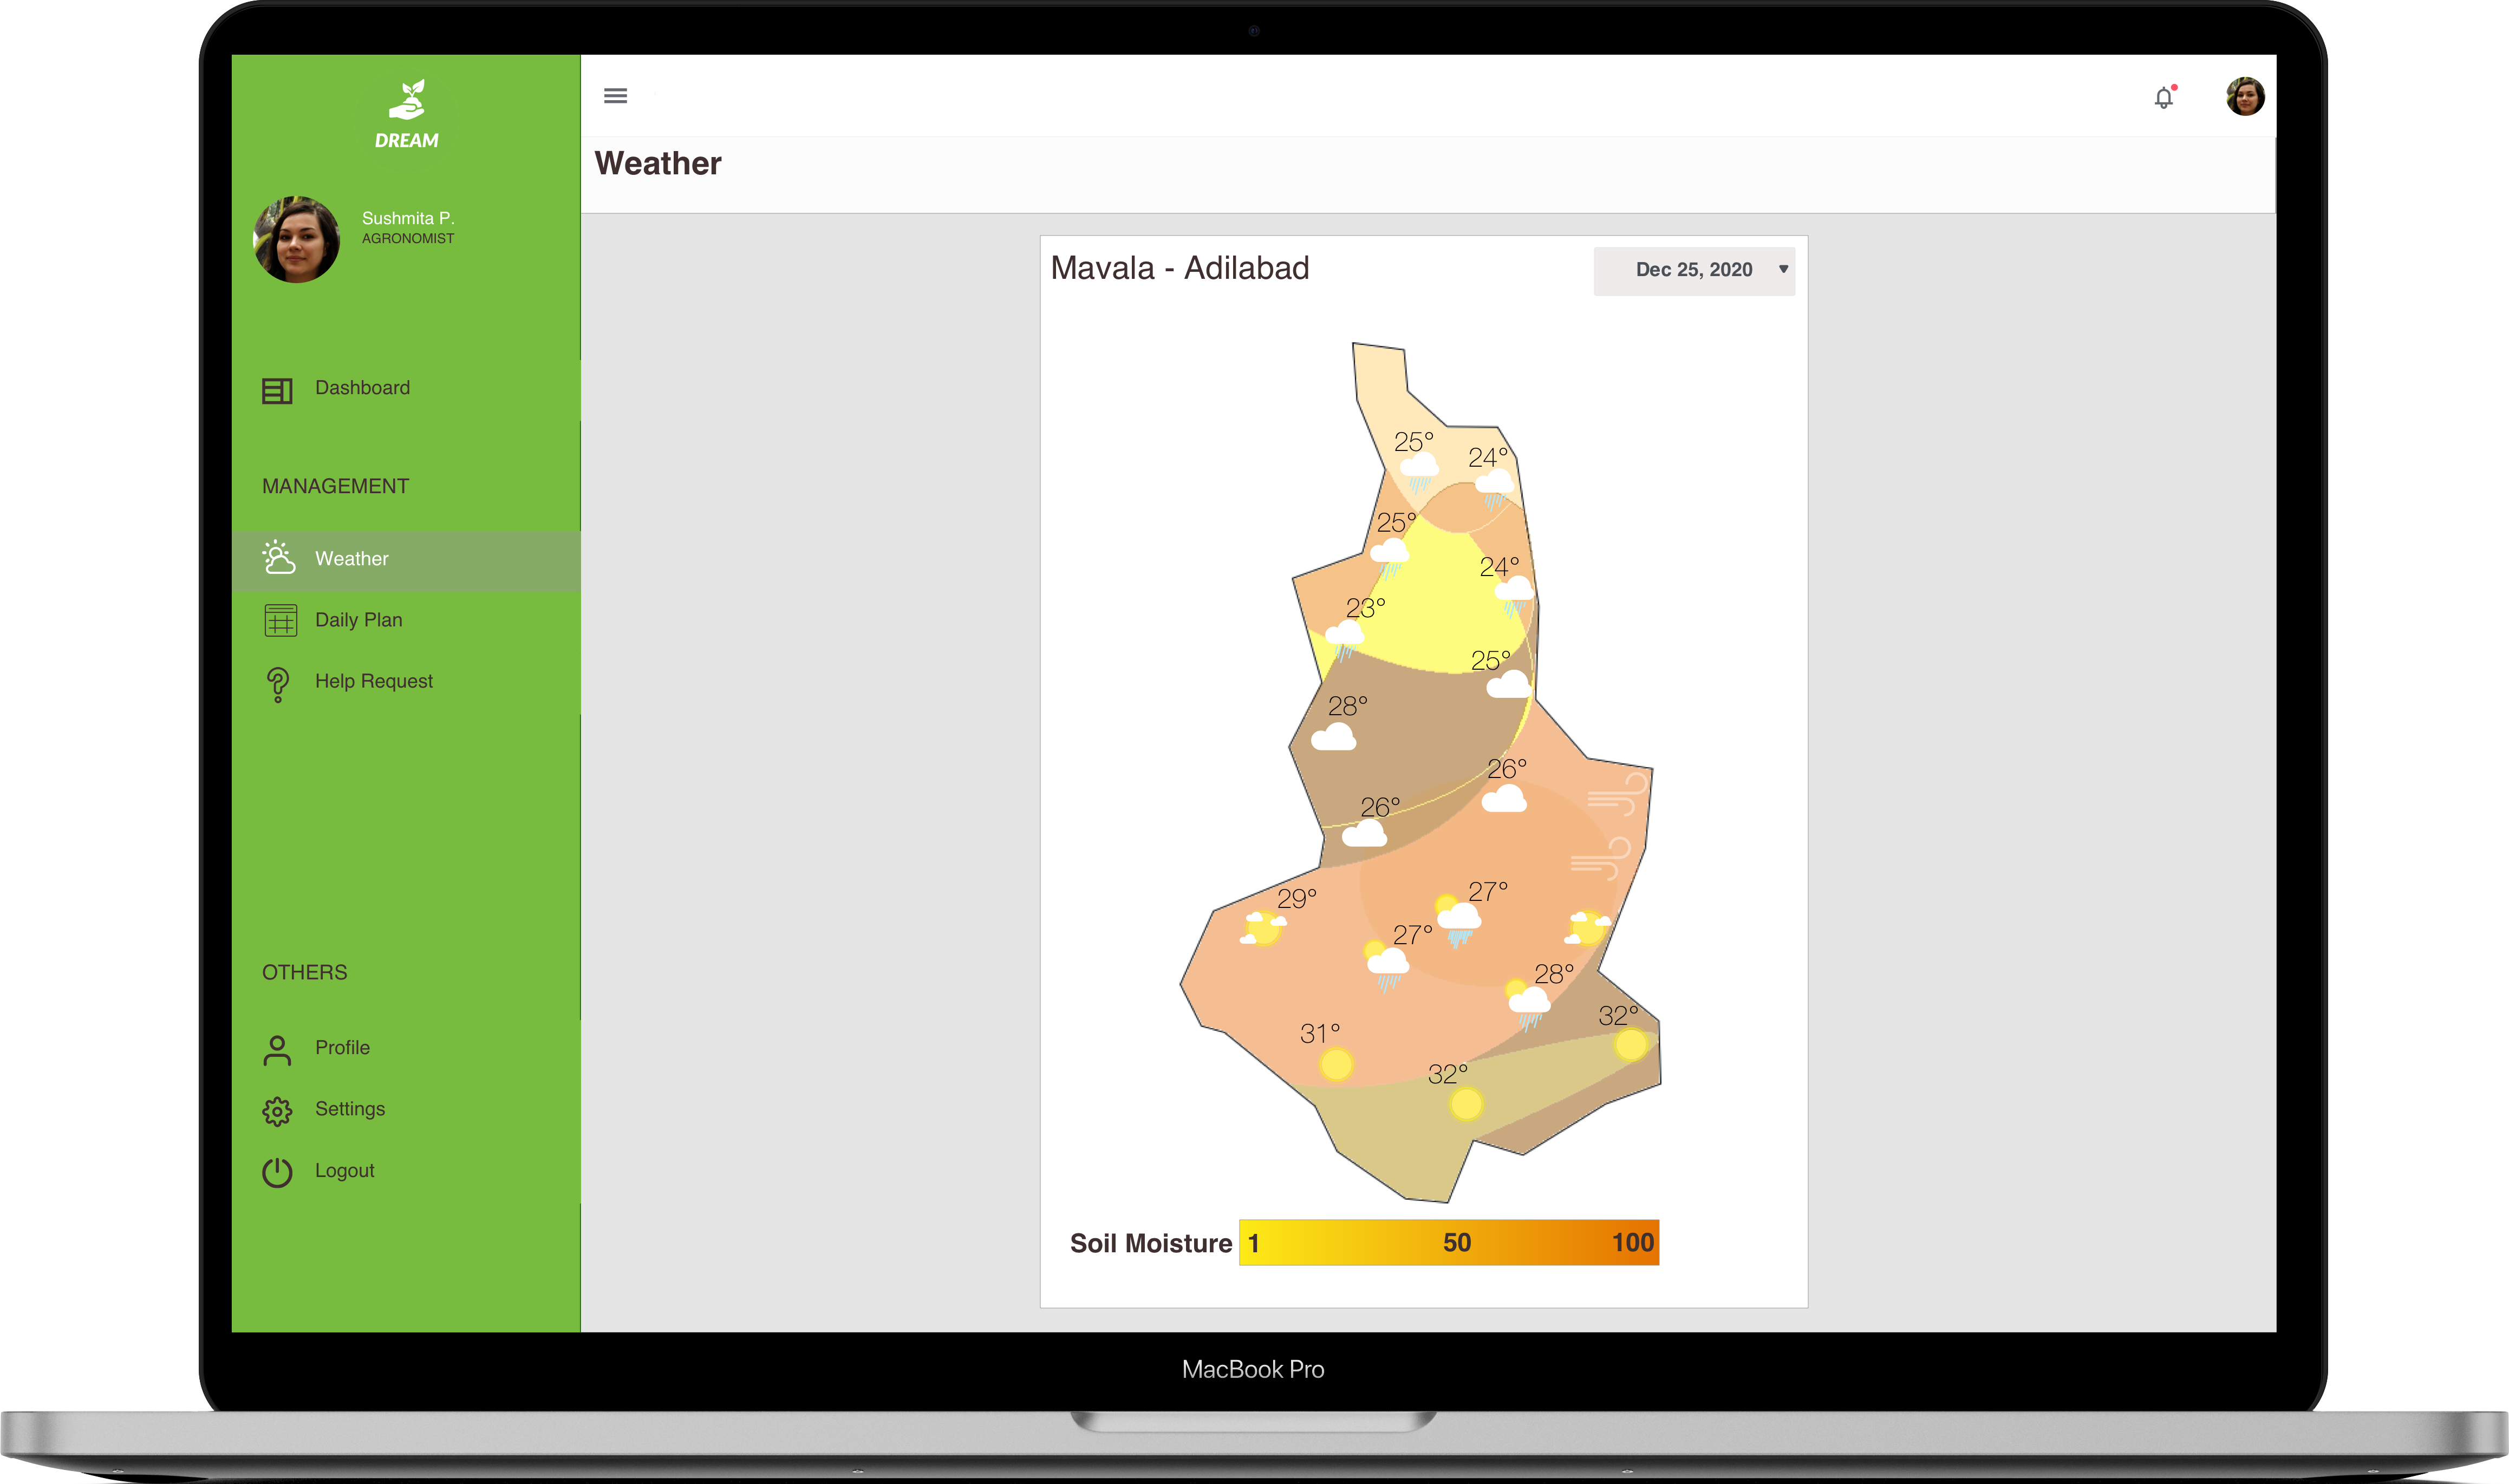
\includegraphics[width=140mm,scale=0.9]{./Images//Mocks/WebApp/Agronomist_Weather.png}
  \caption{Agronomist Weather page}
\end{figure}

\begin{itemize}
    \item \textbf{Agronomist Weather page}\\ 
    \textcolor{red}{This is Agronomist weather page, where he/she can visualize info about weather conditions and soil moisture of his/her mandal. He/she can also view information about weather conditions and soil moisture in the next 7 days by setting it into the menu.}
\end{itemize}


\begin{figure}[H]
  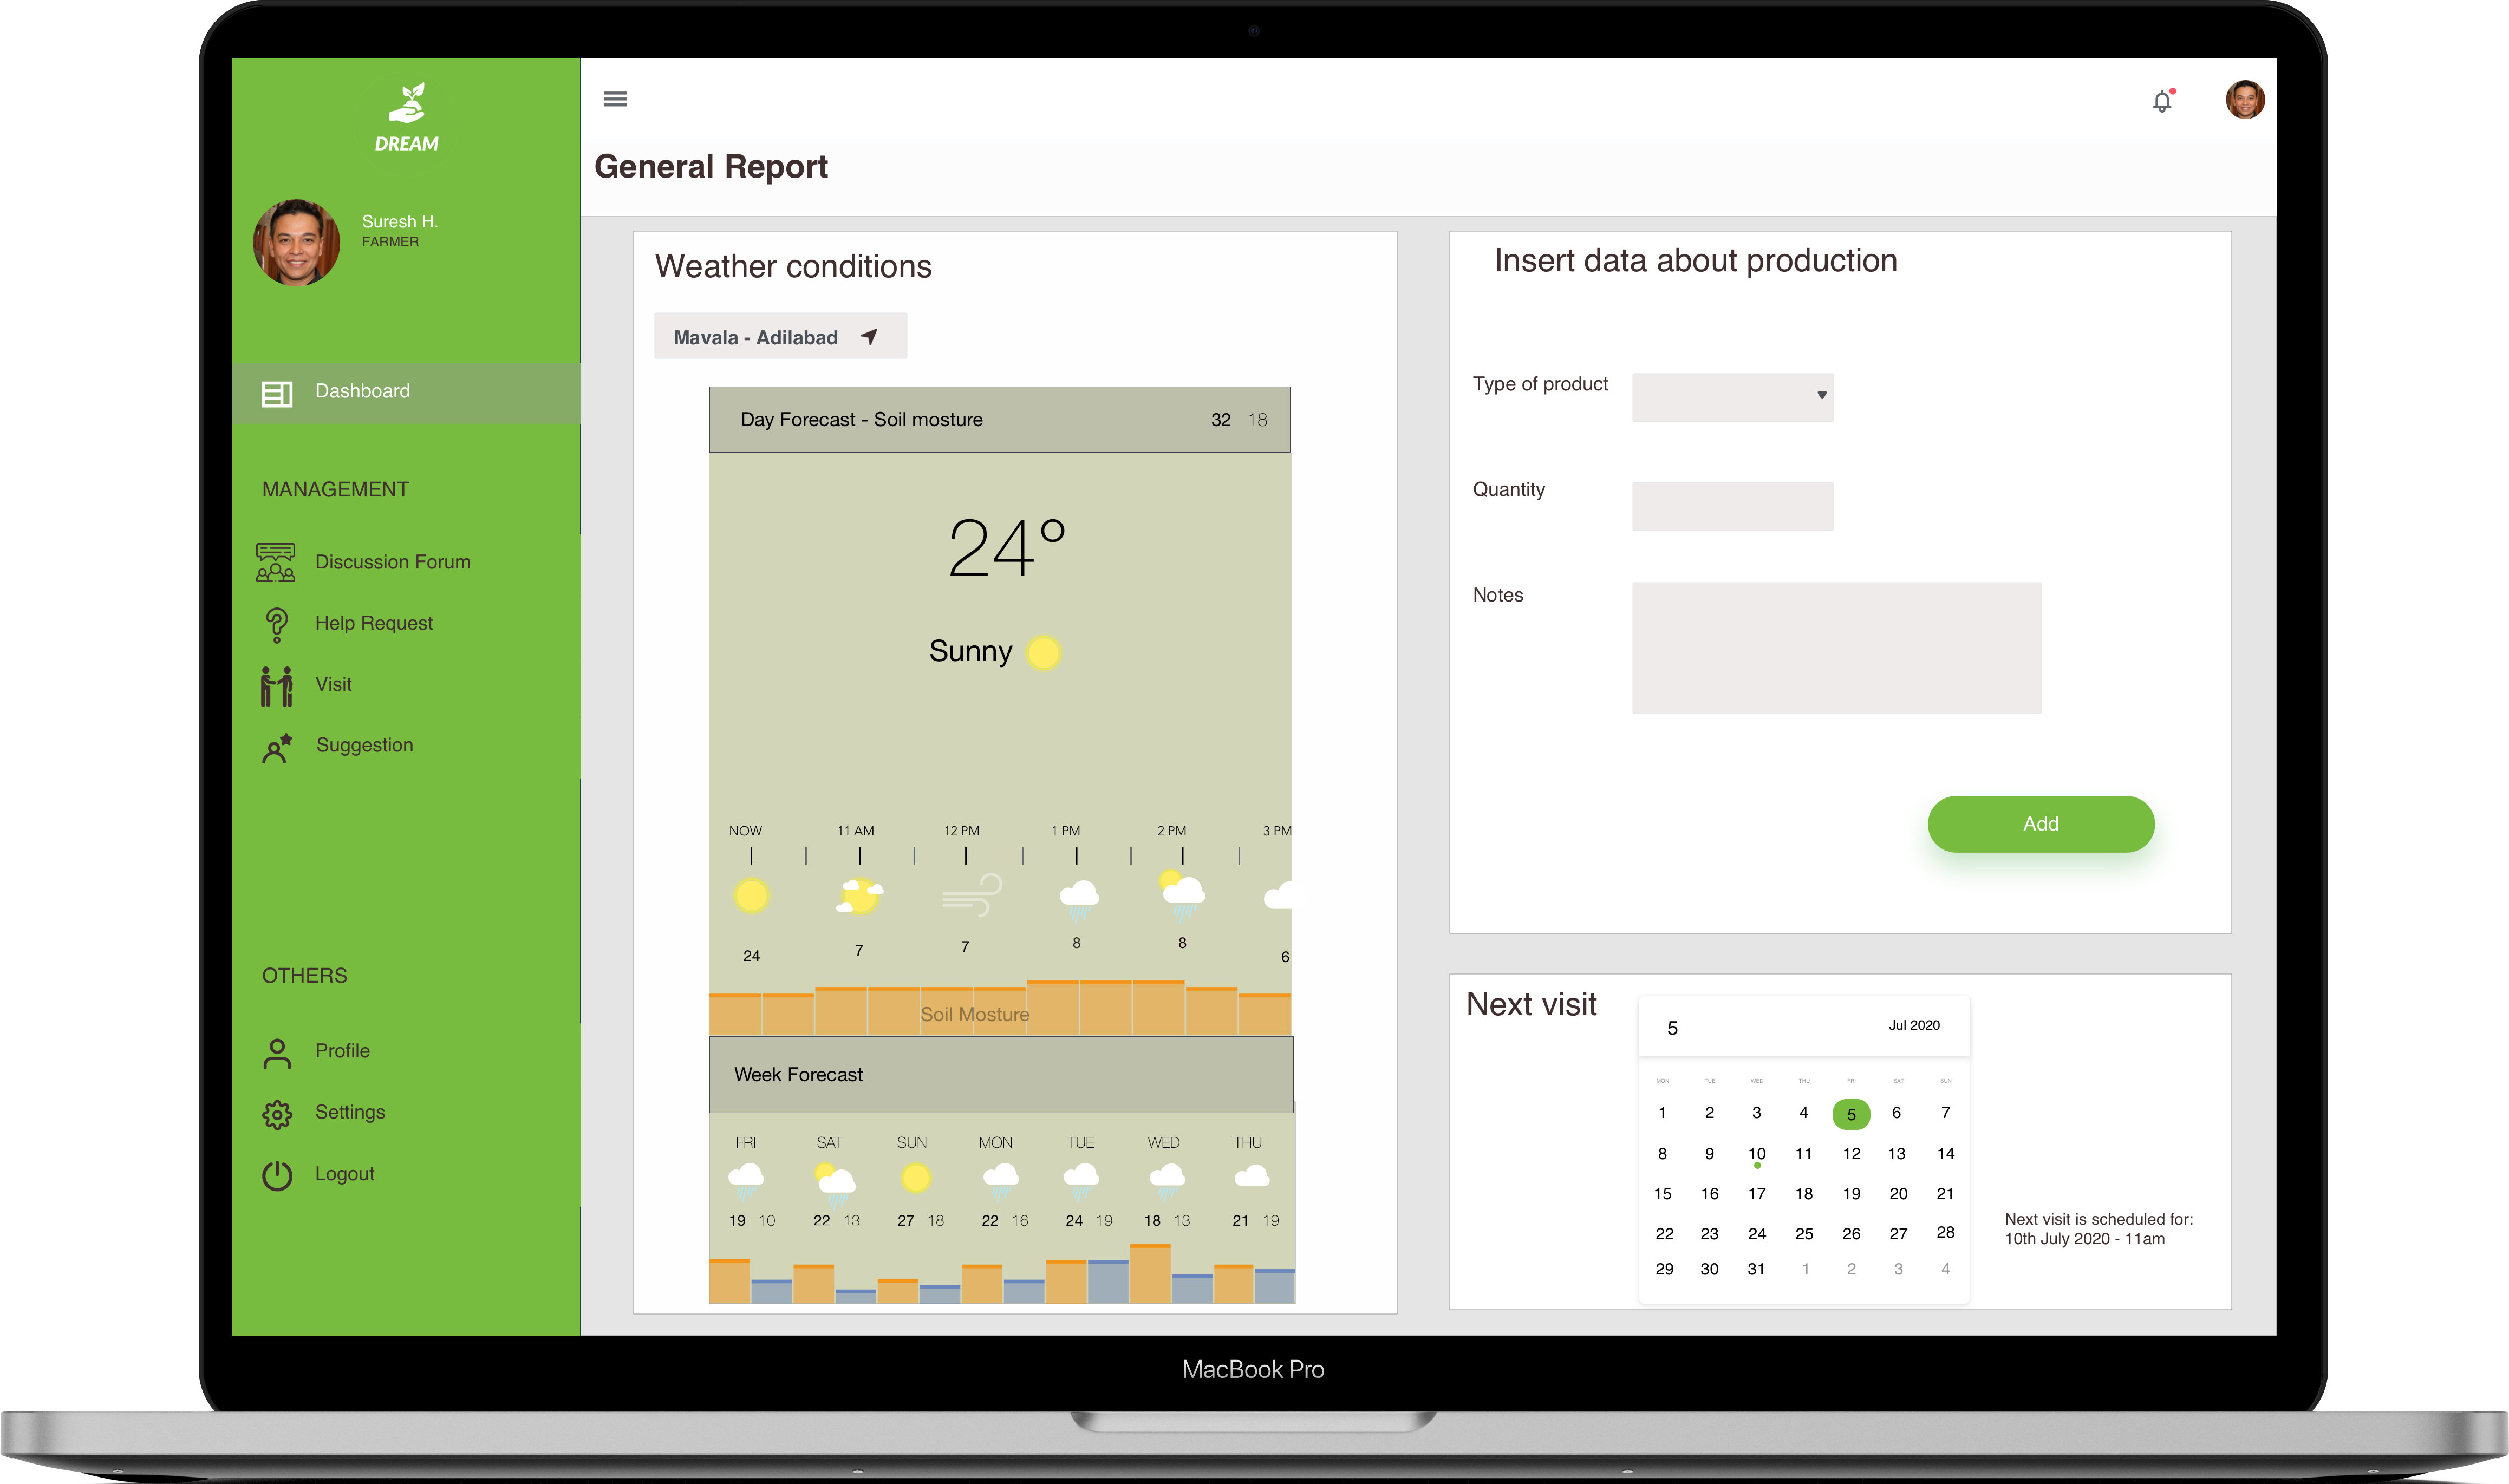
\includegraphics[width=140mm,scale=0.9]{./Images//Mocks/WebApp/Farmer_Home.png}
  \caption{Farmer Home page}
\end{figure}

\begin{itemize}
    \item \textbf{Farmer Home page}\\ 
    \textcolor{red}{This is Farmer homepage (in \textit{Figure 3.6} called "Dashboard") where he/she can visualize weather conditions based on her/his location, he/she can insert data about his/her production and can visualize on the calendar the next visit.}
\end{itemize}


\begin{figure}[H]
  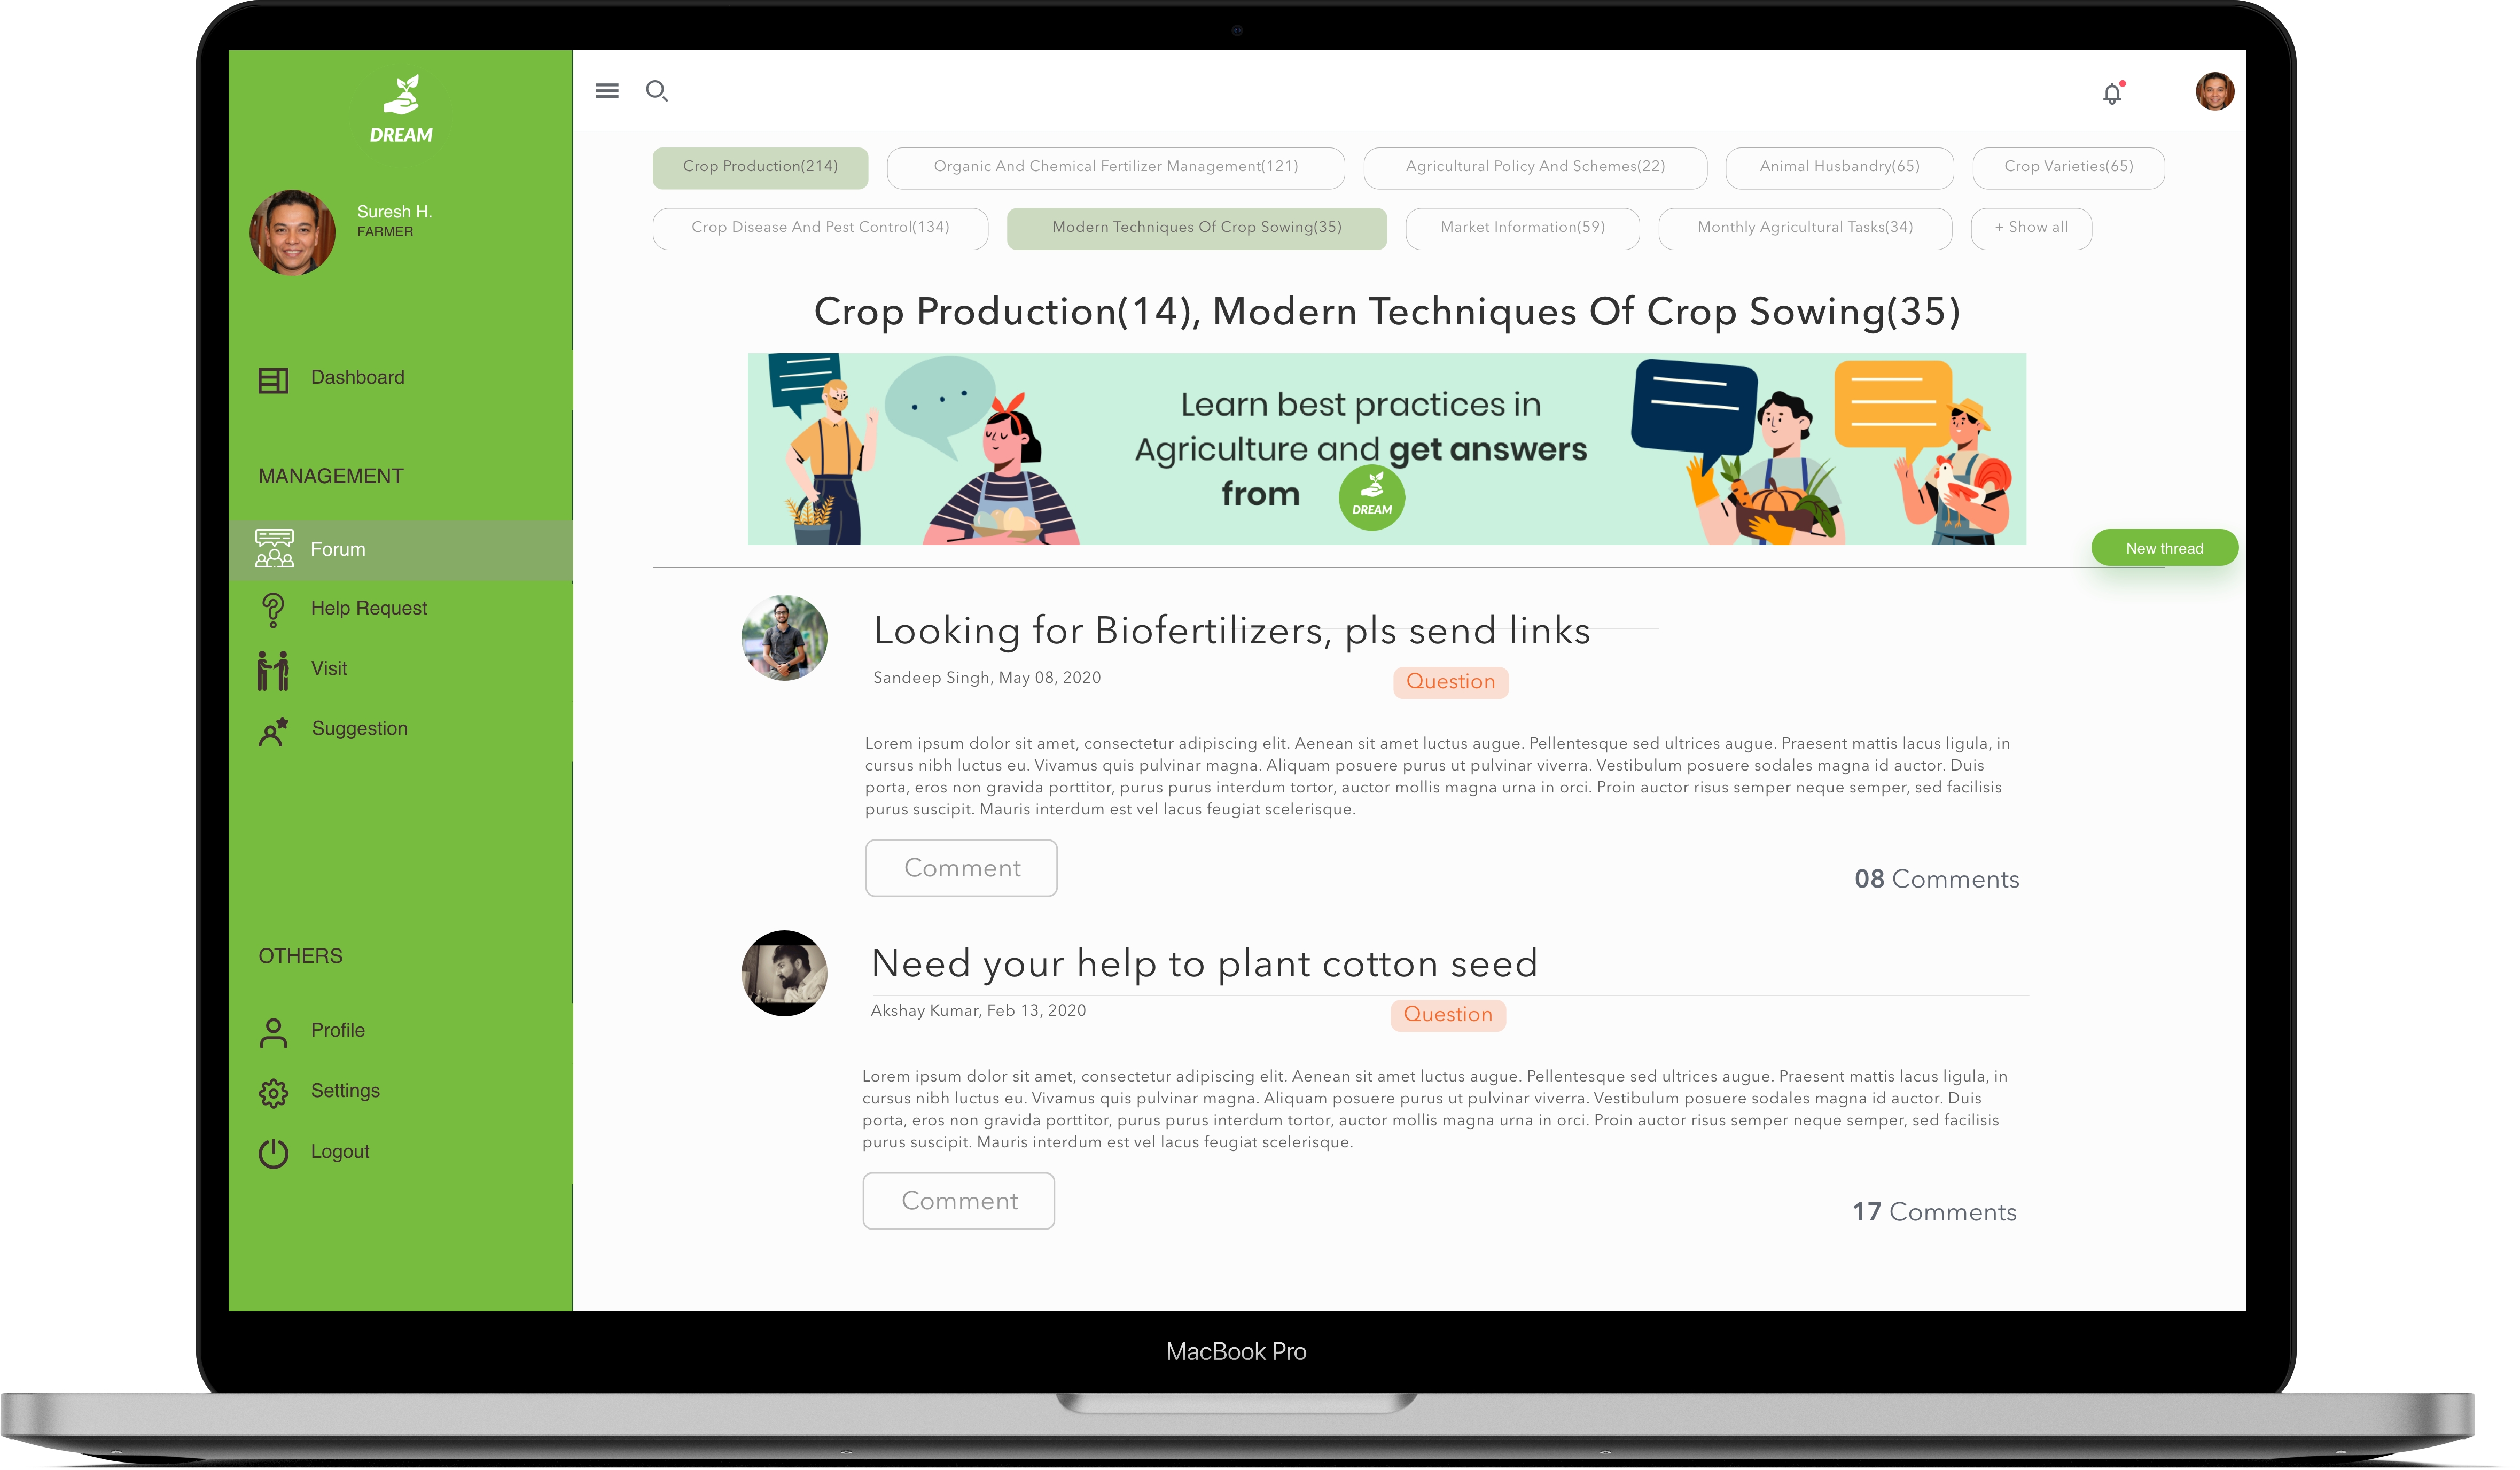
\includegraphics[width=140mm,scale=0.9]{./Images//Mocks/WebApp/Farmer_Forum.png}
  \caption{Farmer Discussion Forum page}
\end{figure}

\begin{itemize}
    \item \textbf{Farmer discussion forum page}\\ 
    \textcolor{red}{This is Farmer forum section, where he/she can interact with other farmers by opening new threads or replying to existing one.
    He/she can also look up for a thread using search function.}
\end{itemize}


\begin{figure}[H]
  \centering
  \begin{minipage}{0.4\textwidth}
    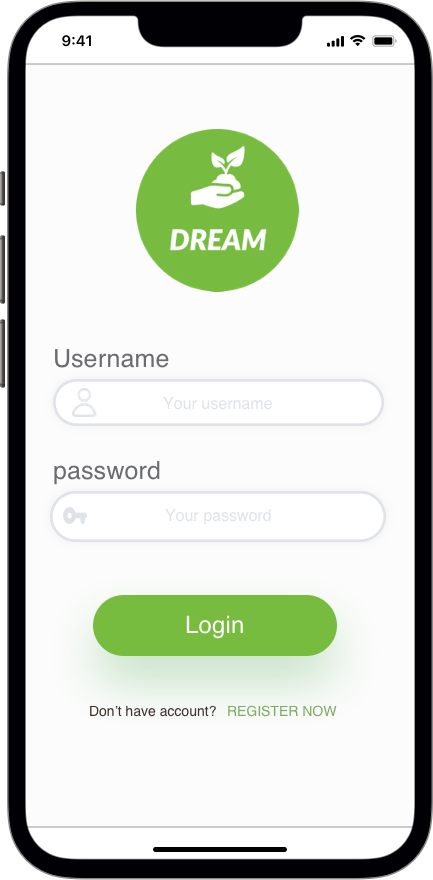
\includegraphics[width=40mm,scale=0.9]{./Images//Mocks/Mobile/Login.png}
    \caption{Mobile Login}
   \end{minipage}
   \hfill
   \begin{minipage}{0.4\textwidth}
     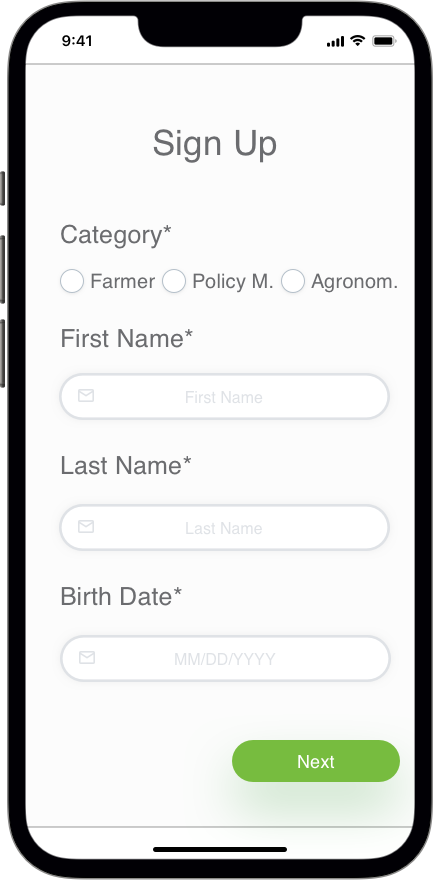
\includegraphics[width=40mm,scale=0.9]{./Images//Mocks/Mobile/Registration.png}
     \caption{Mobile Registration}
   \end{minipage}
\end{figure}


\begin{figure}[H]
  \centering
   \begin{minipage}{0.4\textwidth}
     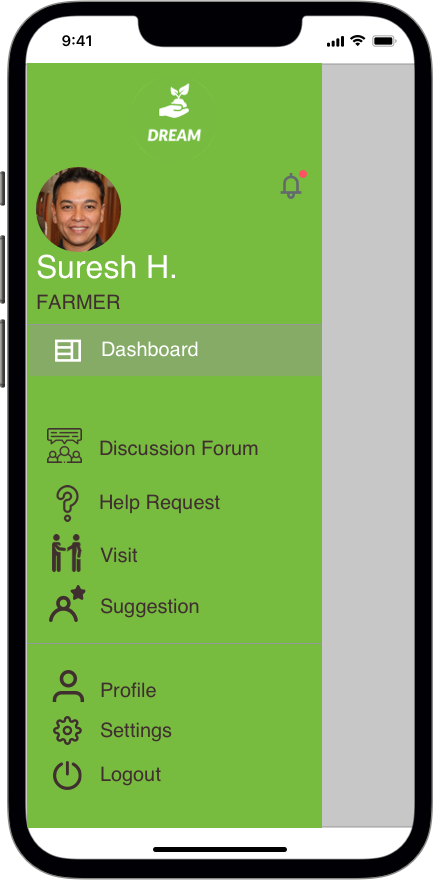
\includegraphics[width=40mm,scale=0.9]{./Images//Mocks/Mobile/Farmer_menu.png}
     \caption{Mobile Farmer menu}
   \end{minipage}
    \hfill
   \begin{minipage}{0.4\textwidth}
     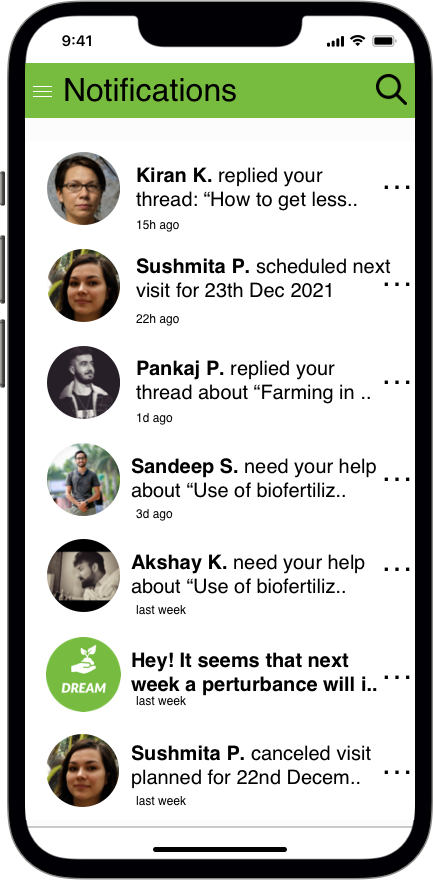
\includegraphics[width=40mm,scale=0.9]{./Images//Mocks/Mobile/Farmer_notif.png}
     \caption{Mobile Farmer notifications}
   \end{minipage}
\end{figure}
\newpage
\begin{itemize}
    \item \textbf{Figure 3.8: Mobile Login}\\ 
    \textcolor{red}{Initial interface, it allows to one of the 3 actors of DREAM to log in by entering their credentials (Username and password). If he/she is not registered, there's a button "REGISTER NOW" to accomplish.
    }
\end{itemize}
\begin{itemize}
    \item \textbf{Figure 3.9: Mobile Registration}\\ 
    \textcolor{red}{Through the registration interface, it is possible to create an account by  one of the three actors of DREAM, by clicking next button other required fields are shown to accomplish the registration.}
\end{itemize}
\begin{itemize}
    \item \textbf{Figure 3.10: Mobile Farmer menu}\\ 
    \textcolor{red}{Interface that shows the menu of actions that a farmer can perform in the application}
\end{itemize}
\begin{itemize}
    \item \textbf{Figure 3.11: Mobile Farmer notifications}\\ 
    \textcolor{red}{Interface that shows various kind of notifications received by a Farmer.}
\end{itemize}
\newpage

\begin{figure}[H]
  \centering
   \begin{minipage}{0.4\textwidth}
     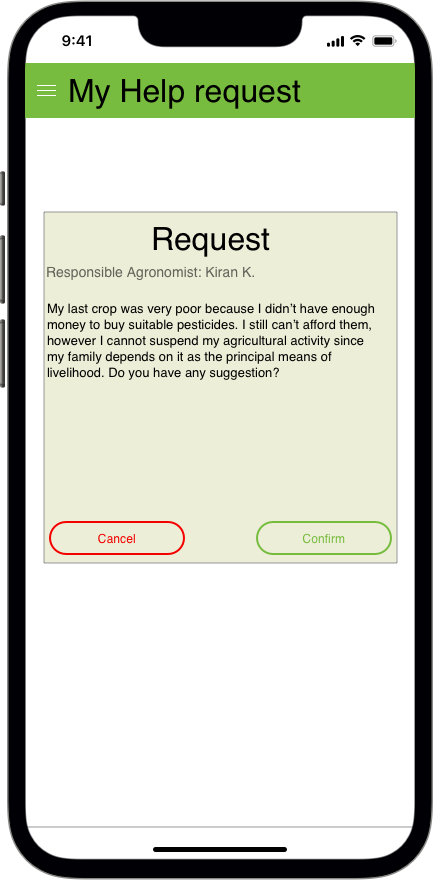
\includegraphics[width=40mm,scale=0.9]{./Images//Mocks/Mobile/Farmer_help_req.png}
     \caption{Mobile Farmer help request}
   \end{minipage}
    \hfill
   \begin{minipage}{0.4\textwidth}
     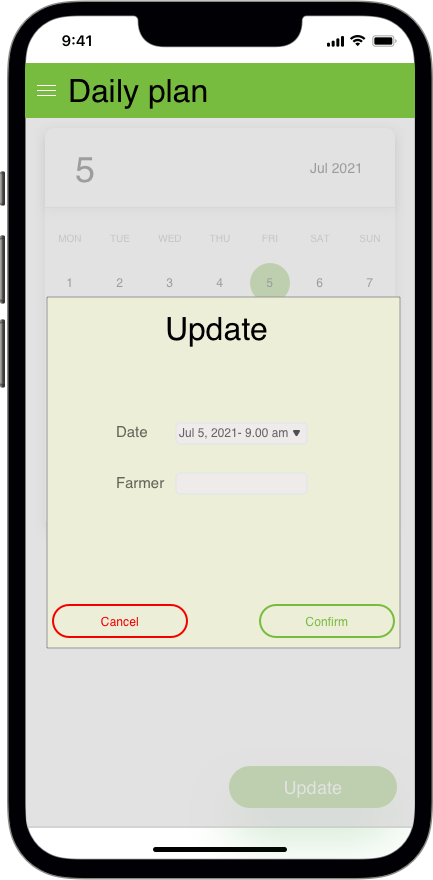
\includegraphics[width=40mm,scale=0.9]{./Images//Mocks/Mobile/Agronomist_daily_plan.png}
     \caption{Mobile Agronomist daily plan}
   \end{minipage}
\end{figure}

\begin{itemize}
    \item \textbf{Figure 3.12: Mobile Farmer help request}\\ 
    \textcolor{red}{Interface that shows an example of help request made by a Farmer to only an Agronomist.}
\end{itemize}
\begin{itemize}
    \item \textbf{Figure 3.13: Mobile Agronomist daily plan}\\ 
    \textcolor{red}{Interface that shows an example of update of the daily plane made by an Agronomist.}
\end{itemize}
\newpage